\section{Indbyggede typer og konstanter}

\begin{frame}
\frametitle{Programmørens omgivelser}
\begin{itemize}
\item Standard Environment
\item Game Environment
\end{itemize}
\end{frame}

\begin{frame}
\frametitle{Standard Environment}
\framesubtitle{Globale konstanter}
\begin{itemize}
\item \constant{typeOf[]} er en funktion, som returnerer et givet objekts type
\item \constant{union[]} er en funktion, som returnerer foreningsmængden af to eller flere lister
\item \constant{true} og \constant{false} er boolske konstanter
\end{itemize}
\end{frame}

\begin{frame}
\frametitle{Standard Environment}
\framesubtitle{Simple typer}
\begin{itemize}
\item \type{Integer}: 32-bit heltal
\item \type{Boolean}: Sandhedsværdi
\item \type{String}: Unicode tekststreng
\end{itemize}
\end{frame}

\begin{frame}
\frametitle{Standard Environment}
\framesubtitle{Lister}
\begin{itemize}
\item En ordnet liste af vilkårlige objekter: \texttt{[\literal{2}, "hej", \constant{true}]}
\item Kan være tom: \texttt{[]}
\item \constant{.size} er listens størrelse
\item Listen kan sorteres med \constant{.sort[]}
\item \constant{.map[]} udfører en funktion på alle listens elementer
\item \constant{.filter[]} returnerer de elementer som opfylder et kriterium
\end{itemize}
\end{frame}

\begin{frame}
\frametitle{Standard Environment}
\framesubtitle{Simple brætspilsrelaterede typer}
\begin{itemize}
\item \type{Coordinate} er en vektor som repræsenterer et felt på et bræt: \literal{C5} og \literal{M27}
\item \type{Direction} er en vektor som repræsenterer et flyt: \literal{n}, \literal{nw} og \texttt{\literal{n} + \literal{ne}}
\item \type{Pattern} er et mønster
\end{itemize}
\begin{center}
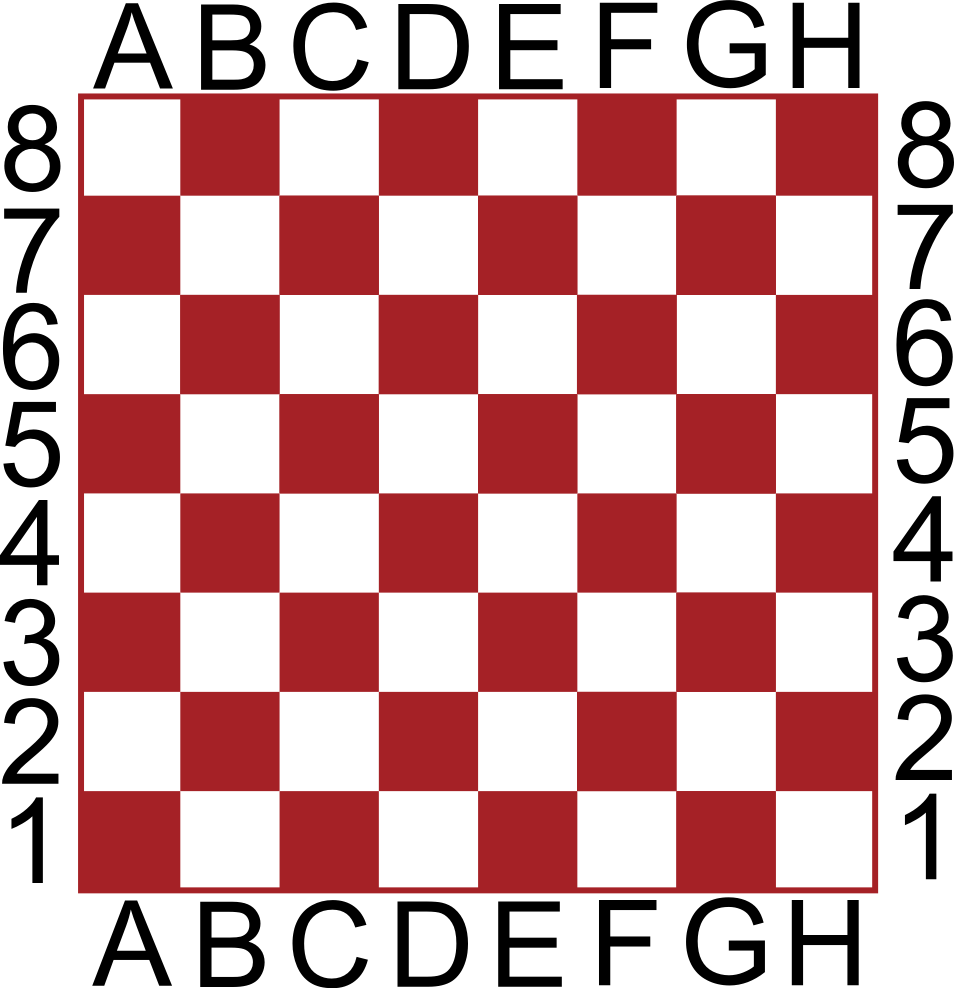
\includegraphics{niels/coordinates.png}
\hspace{0.5cm}

\includegraphics{niels/direction_n.png}
\hspace{0.5cm}
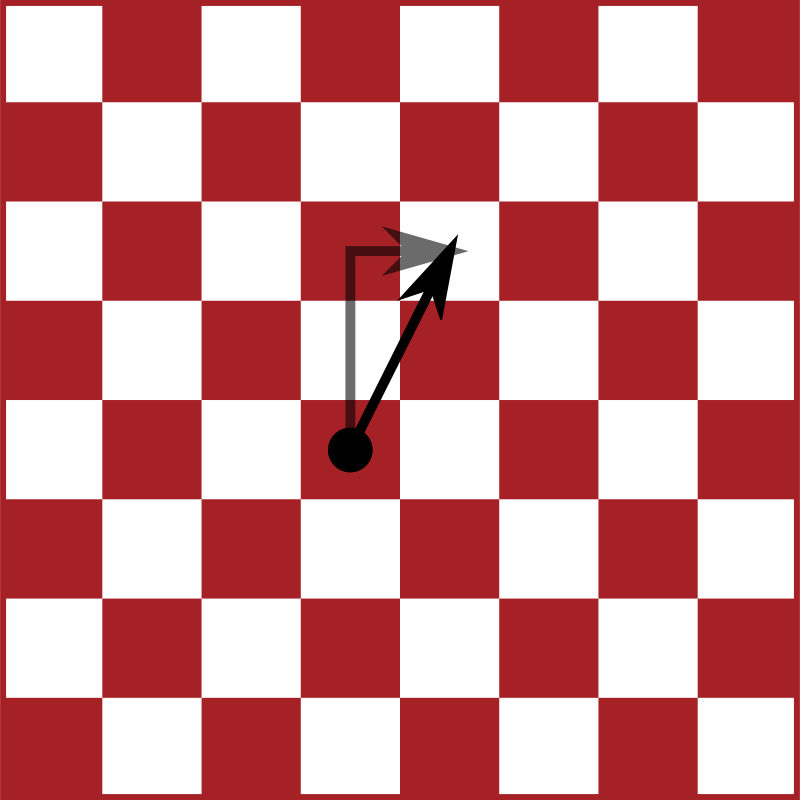
\includegraphics{niels/direction_nne.png}
\end{center}
\end{frame}

\begin{frame}
\frametitle{Standard Environment}
\framesubtitle{Specielle typer}
\begin{itemize}
\item \type{Type} repræsenterer en typeværdi, dette er f.eks. resultatet når man skriver navnet på en type.
\item \type{Function} repræsenterer en funktionsværdi, dette er resultatet når man skriver navnet på en funktion. Eller et lambda-udtryk:
\item \texttt{\#[\variable{a}, \variable{b}] => \variable{a} + \variable{b}}
\end{itemize}
\end{frame}

\begin{frame}
\frametitle{Game Environment}
\begin{itemize}
\item Et klassehieraki til beskrivelse af brætspil.
\item \type{Game}-typen repræsenterer f.eks. et brætspil. Man nedarver fra \type{Game} for at implementere sit brætspil.
\end{itemize}
\begin{center}
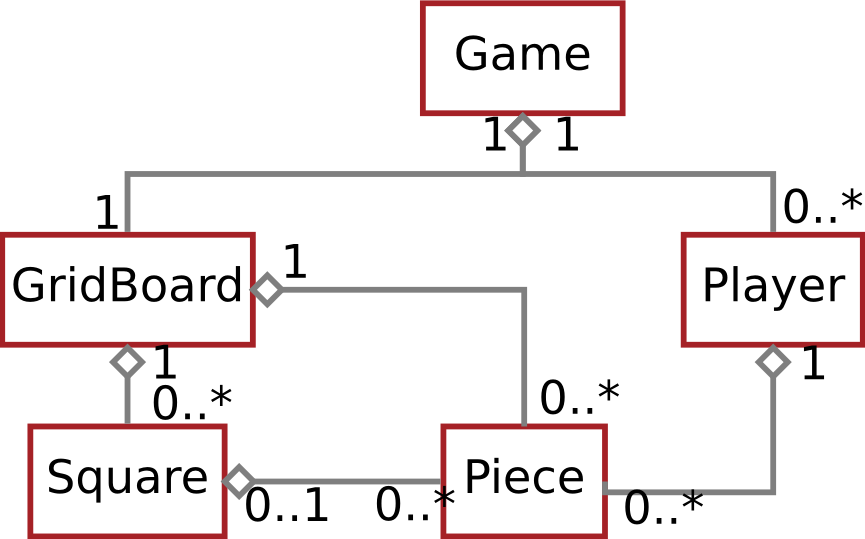
\includegraphics[width=0.7\textwidth]{niels/classes.png}
\end{center}
\end{frame}

\begin{frame}
\frametitle{Game Environment}
\framesubtitle{Actions}
\begin{itemize}
\item Håndtering af tilstandsændringer i brætspil, dvs. træk.
\item F.eks. returner \type{Player}-typens \constant{actions[]}-metode en liste af \type{Action}-objekter, dvs. en liste af mulige træk.
\item \type{AddAction}, \type{RemoveAction} og \type{MoveAction} tillader manipulering af brikker på brættet: Tilføj, fjern, flyt.
\item \type{ActionSequence} tillader kombinering af flere actions.
\end{itemize}
\end{frame}
